\documentclass{beamer}

\usepackage[utf8]{inputenc}
\usepackage[T1]{fontenc}
\usepackage[french]{babel}
\usepackage[ddmmyyyy]{datetime}

\usetheme{Warsaw}
\useinnertheme{rectangles}
\setbeamerfont{headline}{size=\large}
\setbeamerfont{frametitle}{size=\normalsize}

%Plan/Sommaire automatique avant chaque section
\AtBeginSection[]{
  \begin{frame}
  \frametitle{Plan}
  \tableofcontents[currentsection]
  \end{frame}
}

\author{Sonny Klotz - Jean-Didier Pailleux - Malek Zemni}
\institute{UVSQ}
\date{\today}
\usepackage{../tex/myInfolines}
\title{Présentation Cahier des Charges}

\begin{document}

	\begin{frame}
		\titlepage
	\end{frame}
	
	\section{Introduction}
	\begin{frame}
		Projet de L3 informatique UVSQ, remis par DCbrain.\\~\\
		Le travail est décrit dans ce cahier des charges :
		\begin{itemize}
			\item Motivations
			\item Contraintes
			\item Exigences fonctionnelles
			\item Exigences non fonctionnelles
			\item Autres aspects du projet
		\end{itemize}
	\end{frame}
	
	\section{Motivations du projet}
	\begin{frame}
		\textbf{Problème :} masses de données importantes et difficilement exploitables
		\textbf{Objectif :} fournir un outil d'analyses préliminaires de ces données
		\\~\\
		\pause
		\textbf{Parties prenantes :} \pause
		\begin{itemize}
			\item \textbf{Maitre d'ouvrage :} DCbrain, module Projet de l'UVSQ
			\item \textbf{Client :} DCbrain
			\item \textbf{Autres :} industriels
		\end{itemize}
		\begin{center}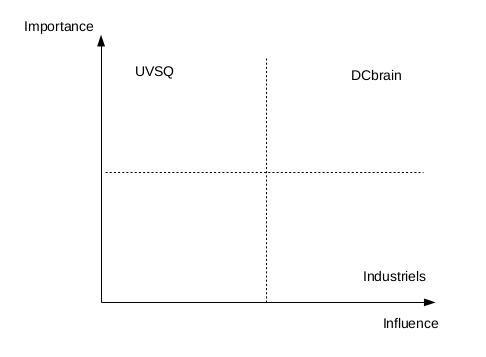
\includegraphics[scale=0.35]{../Cahier/diagPP.png}\end{center}
		\pause \vspace{-0.5em}
		\textbf{Utilisateurs :} membres de DCbrain + industriels du domaine
	\end{frame}	
	
	\section{Contraintes}
	\begin{frame}
		3 exigences contraignantes pour le produit :
		\pause
		\begin{itemize}
			\item Fournir une application web \textbf{\textit{applet}}
			\pause
			\item Développé avec un langage permettant une analyse de données
			\pause
			\item Fournir API d'analyse de données en sortie
		\end{itemize}
		~\\
		\pause
		\textbf{Environnement de fonctionnement :} celui d'une \textbf{\textit{applet}}
			\begin{center}\begin{tikzpicture}[scale=0.5]\begin{scope}[xscale=2,yscale=1.5]	
				\node (USR) at (-3,0) [rectangle,draw] {\begin{tabular}{c}{\tiny Utilisateur}\end{tabular}};
				\node (NAV) at (0,0) [rectangle,draw,fill=blue!25] {\begin{tabular}{c}{\tiny Navigateur web}\end{tabular}};
				\node (APP) at (3,0) [rectangle,draw] {\begin{tabular}{c}{\tiny Application}\end{tabular}};
				\path[->,>=stealth'] (USR) edge[bend left=17] node[anchor=south,above]{{\tiny Accès à l'hôte}} (NAV);
				\path[->,>=stealth'] (NAV) edge[bend left=17] node[anchor=south,above]{{\tiny Intégration de l'application}} (APP);
			\end{scope}\end{tikzpicture}\end{center}
		~\\
		\pause
		\textbf{Applications partenaires :} outils de DCbrain (intégration API)
		\\~\\
		\pause
		\textbf{Temps et budget :} rendu avant le 26/05/2017, aucun budget.
	\end{frame}
	
	\section{Exigences fonctionnelles}
	\begin{frame}
		Sonny
	\end{frame}
	
	\section{Exigences fonctionnelles}
	\begin{frame}
		\begin{center}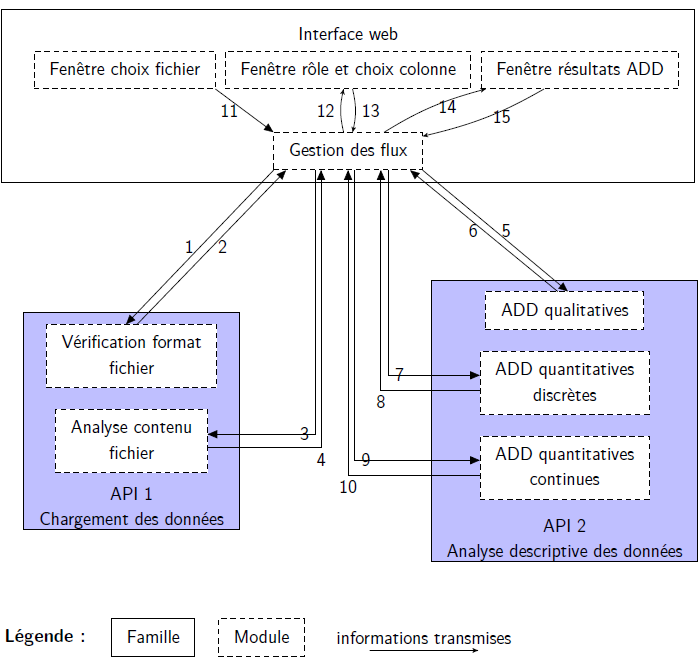
\includegraphics[scale=0.43]{org.png}\end{center}
	\end{frame}
	
	\section{Exigences non fonctionnelles}
	\begin{frame}
		Jean-Édouard
	\end{frame}
	
	\section{Autres aspects}
	\begin{frame}
		Jean-Claude
	\end{frame}
	
	\section{Conclusion}
	\begin{frame}
		Jean-Claude Van Damme
	\end{frame}
	
\end{document}
